\chapter{Analysis of results' quality of AlphaFold-disorder (SASA)}
\label{chp:analysis}
AlphaFold/disorder (SASA) is the variation we developed of the software-tool AlphaFold-disorder, using PSEA and SASA instead of DSSP to compute the predictions, in particular we have the SASA variation for each of the three algorithms within the software-tool:
\begin{itemize}
    \item AlphaFold-pLDDT (SASA);
    \item AlphaFold-rsa (SASA);
    \item AlphaFold-binding (SASA).
\end{itemize}

Now we have to understand if this new software-tool produces good predictions: we need to evaluate the results' quality. To do so, we will analyse the output datasets, which contain the predictions, of AlphaFold-disorder and AlphaFold-disorder (SASA) and compare them to a ground truth:
\begin{itemize}
    \item Analyse the columns of the output datasets;
    \item Create plots or visualizations, to gain insights on the results and patterns between features (statistics and predictions);
    \item Finally create ML models and analyse the statistics and main plots of the best models.
\end{itemize}

\section{Output dataset}
The software-tool produces two output files:
\begin{itemize}
    \item output\_data.tsv: contains the statistics before computing the predictions;
    \item output\_pred.tsv: contains both the statistics and the predictions.
\end{itemize}
We will consider only the latter one, since it includes the first one inside. The name of the files depends on the parameter given by command line when using the software-tool. 

Both in AlphaFold-disorder dataset and AlphaFold-disorder (SASA) dataset we have the same columns, an example of such a dataset in table \ref{tab:dataset}.



Let's continue the analysis by creating a few plots, to visualize any pattern or relationship between columns and gain some insight.

\section{Plots}
We obtained the ground truth from the CAID web application, and we considered the structural features of the proteins present in these ground truths. These ground truths are simply lists of "0", "-" and "1" for each residue in some proteins: 0 when that characteristic is absent, 1 when is present and - when it's uncertain. We described this procedure to obtain and process the CAID ground truths in \ref{analysis-procedures}.

We tried a few different plots, to compare the relationships between the most important features of the datasets: 

\begin{itemize}
    \item lddt;
    \item rsa;
    \item disorder-25;
    \item binding-25.
\end{itemize}

Disorder-25 and Binding-25 are respectively the predictions of AlphaFold-rsa and AlphaFold-binding.

We can categorize the plot we made in two:

\begin{enumerate}
    \item By ground truth used:
        \begin{itemize}
            \item Binding: ground truth on binding, which is basically an array with an annotation for every residue, 1 if it's a residue that binds with other residues or molecules, 0 otherwise;
            \item Disorder: same but on disorder.
        \end{itemize}
    \item By type of plot:
        \begin{itemize}
            \item Density plot;
            \item Histograms;
            \item Jointplot;
            \item Scatterplot.
        \end{itemize}
\end{enumerate}

We made the plots using the Python library \textbf{seaborn}, in particular we used the procedures scatterplot, kdeplot, jointplot and histplot. While the other are obvious, to create density plots we used the kdeplot procedures.

More information on seaborn, on the \href{https://seaborn.pydata.org/}\underline{{website}}.

\vspace{10em}

\subsection{Density plots}
For density plots we have two setups per ground truth: for example for the binding ground truth we created the plot for every feature for residues where ground truth is 0 and another plot with every feature for residues with ground truth 1. We made equivalent plots for the disorder ground truth. Down below a few pictures to illustrate these two types of density plots.

\pagebreak

\begin{figure}[h!]
    
    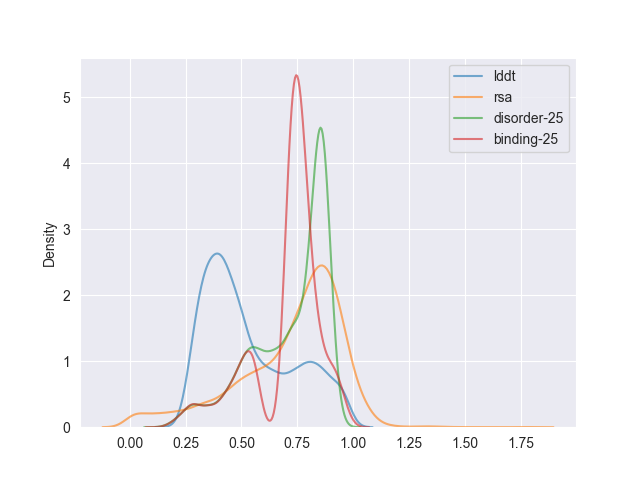
\includegraphics[scale=0.9]{res/analysis/plots/bind1-density_all.png}
    \caption{Density plot}
\end{figure}

This is the density plot of every feature, for the residues with binding ground truth equal to one (positive binding class).

\subsection{Histogram plots}

For histogram plots we made three different types per ground truth:

\begin{enumerate}
    \item Every feature where the ground truth is 0;
    \item Every features when ground truth 1;
    \item For every feature we made a plot comparing values of that feature for residues in the two classes (ground truth=0 and ground truth=1)
\end{enumerate}


I will show one example of each kind of plot: 

\begin{itemize}
    \item Histogram of every feature for one class: every feature is plotted for residues belonging to one class of the ground truth;
    \item Histogram of one feature for both classes: one feature is plotted for the 2 classes of the ground truth, so we can better compare them.
\end{itemize}

For the second type of histogram plot, I decided to show it for the RSA feature with the disorder ground truth.

\begin{figure}[h!]
\centering
    \begin{subfigure}{0.8\linewidth}
        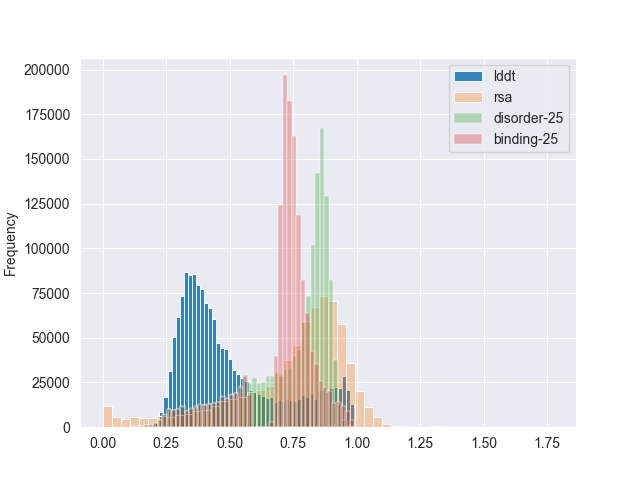
\includegraphics[width=\linewidth]{res/analysis/plots/dis1-histplot_all.png}
        \caption{Histogram plot: every feature}
    \end{subfigure}
    \vfill
    \begin{subfigure}{0.8\linewidth}
        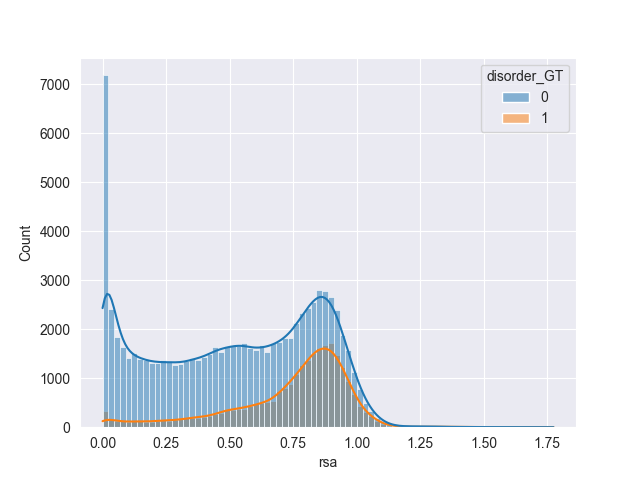
\includegraphics[width=\linewidth]{res/analysis/plots/hue-histplot_rsa.png}
        \caption{Histogram plot: RSA feature}
    \end{subfigure}

\end{figure}

These plots are on the disorder ground truth, we made equivalent plots for the binding ground truth too.

\subsection{Scatter plots}

I will show the scatter plots of the pair (rsa, lddt) for binding ground truth.

\begin{figure}[h!]
    \centering
    \begin{subfigure}{0.8\linewidth}
        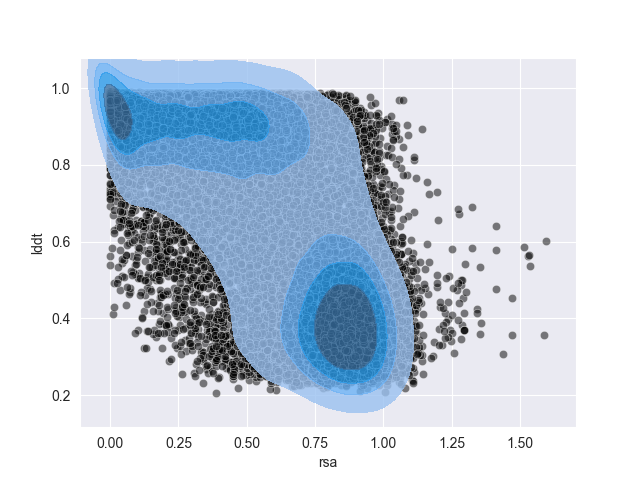
\includegraphics[width=\linewidth]{res/analysis/plots/bind0-scatter_rsa-lddt.png}
        \caption{Scatterplot (rsa, lddt) - positive class}
    \end{subfigure}
    \vfill
    \begin{subfigure}{0.8\linewidth}
        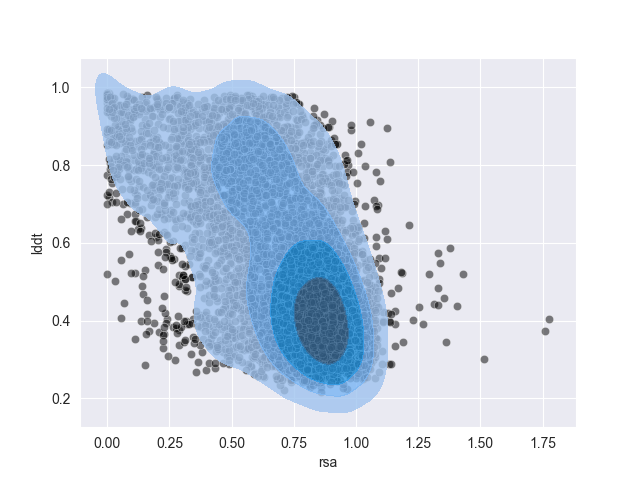
\includegraphics[width=\linewidth]{res/analysis/plots/bind1-scatter_rsa-lddt.png}
        \caption{Scatterplot (rsa, lddt) - negative class}
    \end{subfigure}
\end{figure}

We made four scatter plot for each pair of features: two per ground truth, one for the positive class and one for the negative class.

The possible pairs for our four features are: 

\begin{itemize}
    \item (rsa, lddt);
    \item (rsa, binding-25);
    \item (rsa, disorder-25);
    \item (lddt, binding-25);
    \item (lddt, disorder-25);
    \item (disorder-25, binding-25).
\end{itemize}

For every pair we made two plots per ground truth:

\begin{itemize}
    \item Scatter plot for positive class: only data points belonging to the positive class of the ground truth are considered;
    \item Scatter plot for negative class.
\end{itemize}

We can see some sort of correlation from the scatter plots of rsa and lddt. Although we don't see much of a difference between negative and positive class, which means the correlation between rsa and lddt doesn't depend much from the binding.

\vspace{10em}


\subsection{Joint plots}
The joint plots are made with the same logic of scatter plots: four plots for every pair of features (one plot for positive class and one for negative of each ground truth).

Let's see an example of joint plot, a joint plot of the pair (rsa, lddt) for the positive class of the disorder ground truth.

\begin{figure}[h!]
    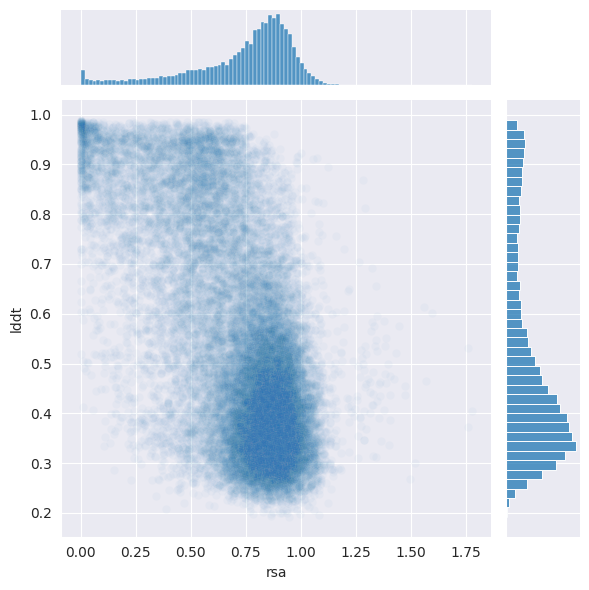
\includegraphics[width=\linewidth]{res/analysis/plots/dis1-jointplot_rsa-lddt.png}
    \caption{Jointplot (rsa, lddt) - postive class for disorder ground truth}
\end{figure}


\subsection{Interpretation of Plots}
We made thirty-eight plots compared to the binding ground truth and another thrirty-eight compared to the disorder one. 

We can clearly see that there is some correlation between the features, we can confirm that disorder and lddt are strictly correlated, and that rsa is correlated both with disorder and binding. 

To further explore and better evaluate the results, we decided to develop a few ML model and compare the precision-recall and ROC plots to the benchmark ones (AlphaFold-plddt, AlphaFold-rsa and AlphaFold-binding).

\section{ML models}
For the machine learning models we considered two different ground truths for disorder and one for binding:
\begin{itemize}
    \item disorder-pdb;
    \item disorder-nox;
    \item binding.
\end{itemize}
these three ground truths are from the CAID web application. We described the procedure to obtain and process the CAID ground truths in \ref{analysis-procedures}.

We developed machine learning models using the three ground truths as target features for the test datasets: so we will have three test datasets, based on the ground truth used and one train dataset, where the target feature will be either binding or disorder, based on the test dataset used.

Let's analyse the preprocessing steps we made.

\vspace{5em}

\subsection{Preprocessing}
As test datasets we used the dataframes containing the proteins present in each of the ground truths, with target the ground truths.

While as train dataset we used the dataframe of all the proteins in the DisProt database, using as target either the disorder or binding functional annotations present in DisProt, based on the test dataset used. We described the procedure to obtain these proteins and these functional annotations from DisProt in \ref{analysis-procedures}.

We computed a one-hot encoding of the ss column: \textbf{ss\_onehot}, so we have a number instead of characters "H", "E", "C". We did this both for test datasets and for train datasets. 

We also added new features to improve the accuracy of ML models: we incorporated the Atchley scale in the datasets. This Atchley scale consists in five features that are defined for each residue.

\pagebreak

\begin{table}[h!]
    \centering
    \setlength{\tabcolsep}{1.2em}
    \fontsize{12pt}{12pt}\selectfont
    \begin{tabular}{c c c c c c}
        \textbf{Amino} & \textbf{Factor} & \textbf{Factor} & \textbf{Factor} & \textbf{Factor} & \textbf{Factor} \\
        \textbf{acid} & \textbf{I} & \textbf{II} & \textbf{III} & \textbf{IV} & \textbf{V} \\
        \hline
        \\
         A & -0.591 & -1.302 & -0.733 & 1.570 & -0.146 \\ 
         C & -1.343 & 0.465 & -0.862 & -1.020 & -0.255 \\
         D & 1.050 & 0.302 & -3.656 & -0.259 & -3.242 \\
         E & 1.357 & -1.453 & 1.477 & 0.113 & -0.837 \\
         F & -1.006 & -0.590 & 1.891 & -0.397 & 0.412 \\
         G & -0.384 & 1.652 & 1.330 & 1.045 & 2.064 \\
         H & 0.336 & -0.417 & -1.673 & -1.474 & -0.078 \\
         I & -1.239 & -0.547 & 2.131 & 0.393 & 0.816 \\
         K & 1.831 & -0.561 & 0.533 & -0.277 & 1.648 \\
         L & -1.019 & -0.987 & -1.505 & 1.266 & -0.912 \\
         M & -0.663 & -1.524 & 2.219 & -1.005 & 1.212 \\
         N & 0.945 & 0.828 & 1.299 & -0.169 & 0.933 \\
         P & 0.189 & 2.081 & -1.628 & 0.421 & -1.392 \\
         Q & 0.931 & -0.179 & -3.005 & -0.503 & -1.853 \\
         R & 1.538 & -0.055 & 1.502 & 0.440 & 2.897 \\
         S & -0.228 & 1.399 & -4.760 & 0.670 & -2.647 \\
         T & -0.032 & 0.326 & 2.213 & 0.908 & 1.313 \\
         V & -1.337 & -0.279 & -0.544 & 1.242 & -1.262 \\
         W & -0.595 & 0.009 & 0.672 & -2.128 & -0.184 \\
         Y & 0.260 & 0.830 & 3.097 & -0.838 & 1.512 \\
    \end{tabular}
    \caption{Atchley scale}
\end{table}

As the last step of preprocessing, we defined which features do we want to consider in the learning process and which one is the target. 

For both the train and test datasets we consider as input features:
\begin{itemize}
    \item lddt;
    \item rsa;
    \item ss\_onehot;
    \item the five factors from the Atchley scale.
\end{itemize}
For the train datasets we consider as target feature the DisProt functional annotation, either binding or disorder annotation. In case we used as test dataset the one with target \textbf{binding ground truth}, we will use as target feature for the train set the binding functional annotations of DisProt, otherwise we will use as target feature the disorder functional annotations.

For the test datasets we consider as target feature either of the three ground truths.

\subsection{Development of Machine Learning Models}
For the development of the ML models we implemented the library \textbf{sklearn}, further details on the \href{https://scikit-learn.org/stable/}{\underline{website}}.

The ML task we considered is regression, because we want to obtain the propensity of disorder or binding of the residues.

We implemented eight different ML models: svm, ridge, lasso, poisson-glm, tweedie, k-nearest neighbors, decision tree and extra tree. 

In general to implement the libraries and compute the ML models we used the procedures provided by the library, in particular:
\begin{itemize}
    \item fit(): this procedure allows us to fit the model with our train dataset;
    \item predict(): this procedure allows us to predict a value, given the input data of the test dataset. Then we will compare this value with the target value of the test dataset and evaluate the ML model performances.
\end{itemize}
We also have a class contructor to initialize each model, always provided by the library.

In the code snippets of the various ML models we will see the variables:
\begin{itemize}
    \item \textbf{X\_train}: input features of the train dataset;
    \item \textbf{y\_train}: target feature of the train dataset;
    \item \textbf{X\_test}: input features of the test dataset;
    \item \textbf{y\_pred}: predicted values for output feature, given X\_test.
\end{itemize}

Now I will show the different ML models and how we implemented them with the \textbf{sklearn} library.

\subsubsection{SVM}
Support Vector Machines are one of the most simple yet powerful machine learning models. The objective is find an N-dimensional hyperplane that clearly separates data points of different classes.

\begin{figure}
    \centering
    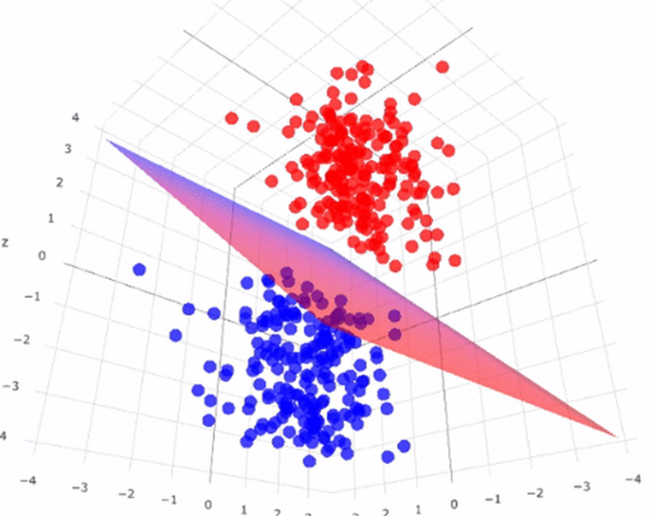
\includegraphics[scale=0.6]{res/ML/svm.png}
    \caption{Picture of SVM hyperplan}
\end{figure}

Let's see now the code snippet of its implementation on a Python notebook.

\begin{lstlisting}[language=Python, caption=SVM implementation]
from sklearn.linear_model import *
[...]
clf = SGDRegressor()
clf.fit(X_train,y_train)
y_pred = clf.predict(X_test)
\end{lstlisting}

The class SGDRegressor is defined in the module \textbf{linear\_model} of sklearn, SGDRegressor stands for Stochastic Gradient Descent because the SVM hyperplane is computed with stochastic gradient descent. This is the most basic linear model for regression.

\subsection{Ridge}
Ridge Regression, also known as Tikhonov regularization or L2 regularization, is a variation of linear regression: it adds a regularization term to make the model more robust.

The L2 regularization discourages large coefficient values: the larger the coefficient the more the regularization term penalizes the model. This makes the model more simple and stable, penalizing complex models.

\begin{lstlisting}[language=Python, caption=Ridge implementation]
from sklearn.linear_model import *
[...]
clf = RidgeCVRegressor()
clf.fit(X_train,y_train)
y_pred = clf.predict(X_test)
\end{lstlisting}

Here we used the \textbf{RidgeCV} class instead of simply \textbf{Ridge}, because we have cross-validation included too, which might increase performances. RidgeCV is also inside the module linear\_model of sklearn.

\subsection{LASSO}
LASSO, Least Absolute Shrinkage and Selection Operator, is a linear regression model which uses L1 regularization. L1 regularization has the effect of setting some of the coefficients to exactly zero. This has the interesting property of performing feature selection, meaning that LASSO can be used to automatically select a subset of the most relevant features.

This is the ML model with better performances with our datasets, probably this automatic feature selection is very effective in our case.

Let's move on to the implementation.

\begin{lstlisting}[language=Python, caption=LASSO implementation]
from sklearn.linear_model import *
[...]
clf = LassoCV()
clf.fit(X_train,y_train)
y_pred = clf.predict(X_test)
\end{lstlisting}

LassoCV is also inside the module linear\_model of sklearn. Even here the cross-validation is included.
\subsection{Poisson GLM}

Poisson Generalized Linear Model is a statistical model used for analyzing count data, where the data follows a Poisson distribution. 

\begin{lstlisting}[language=Python, caption=Poisson-GLM implementation]
from sklearn.linear_model import *
[...]
clf = PoissonRegressor()
clf.fit(X_train,y_train)
y_pred = clf.predict(X_test)
\end{lstlisting}

PoissonRegressor is also inside the module linear\_model of sklearn.
\subsection{Tweedie GLM}

Tweedie Generalized Linear Model is a statistical model used modeling data that follows a Tweedie distribution. 

\begin{lstlisting}[language=Python, caption=Tweedie-GLM implementation]
from sklearn.linear_model import *
[...]
clf = TweedieRegressor()
clf.fit(X_train,y_train)
y_pred = clf.predict(X_test)
\end{lstlisting}

TweedieRegressor is also inside the module linear\_model of sklearn.

\subsection{K-Nearest Neighbors}

K Nearest Neighbors is a regression model that makes predictions based on the average of nearby data points.

\begin{figure}
    \centering
    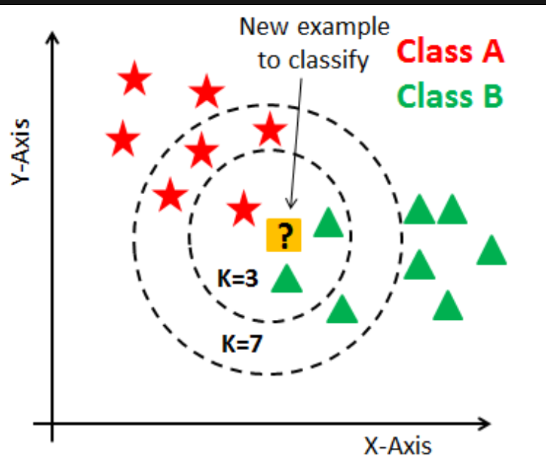
\includegraphics[scale=0.6]{res/ML/knn.png}
    \caption{How KNN algorithm works}
\end{figure}

\begin{lstlisting}[language=Python, caption=K Nearest Neighbors implementation]
from sklearn import neighbors
[...]
clf = neighbors.KNeighborsRegressor()
clf.fit(X_train,y_train)
y_pred = clf.predict(X_test)
\end{lstlisting}

KNeighborsRegressor is defined in the module \textbf{neighbors} of the sklearn library.

\subsection{Decision Tree}
The decision tree splits the dataset into subsets based on the most significant feature, the split points are chosen to minimize the variance for regression. The process is then repeated for each subset, creating a tree-like structure.

To make predictions, the decision tree is traversed from the root to a leaf node, and the value associated with that leaf node is used as the final prediction. During the traversal, the algorithm evaluates the feature at each internal node based on the input features.

\begin{figure}
    \centering
    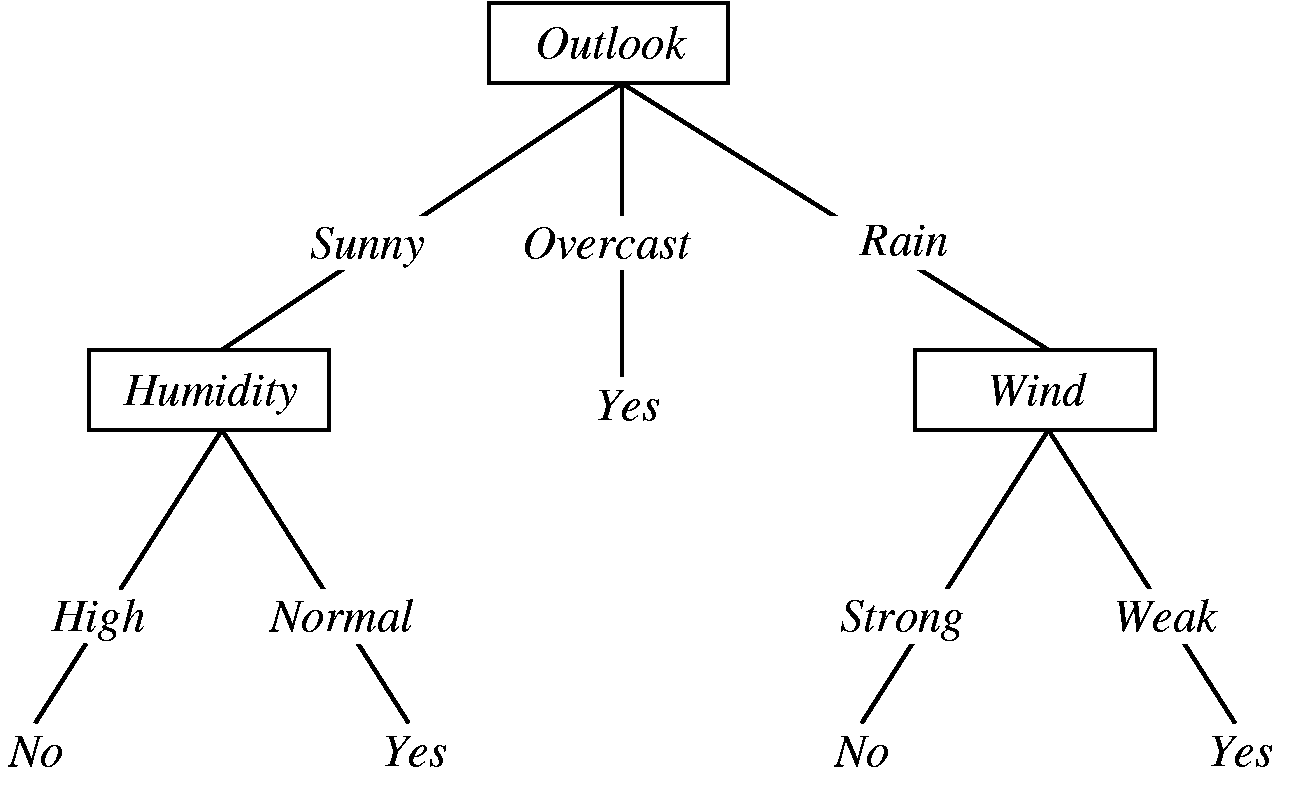
\includegraphics[scale=0.3]{res/ML/decisiontree.png}
    \caption{Example of a decision tree}
\end{figure}

\begin{lstlisting}[language=Python, caption=Decision Tree implementation]
from sklearn import tree
[...]
clf = tree.DecisionTreeRegressor()
clf.fit(X_train,y_train)
y_pred = clf.predict(X_test)
\end{lstlisting}

DecisionTreeRegressor is defined in the module \textbf{tree} of the sklearn library.

\pagebreak

\subsection{Extra Tree}
The extra tree is a combination of multiple decision trees, extremely randomized, to improve the performances and robustness of decision trees.

ExtraTreeRegressor is defined in the module \textbf{tree} of the sklearn library.

\begin{lstlisting}[language=Python, caption=Extra Tree implementation]
from sklearn import tree
[...]
clf = tree.ExtraTreeRegressor()
clf.fit(X_train,y_train)
y_pred = clf.predict(X_test)
\end{lstlisting}




\section{Evaluation of ML models' predictions}

To evaluate the predictions of the ML models, we computed their ROC and Precision-Recall curves and compared them with the ROC and Precision-Recall curves of the software-tools AlphaFold-disorder and AlphaFold-disorder (SASA).

We will see the ROC curves and the Precision-Recall curves divided by ground truth used in the ML models training process.

\vspace{5em}

\pagebreak

\subsection{Disorder PDB}

\begin{figure}[h!]
    \centering
    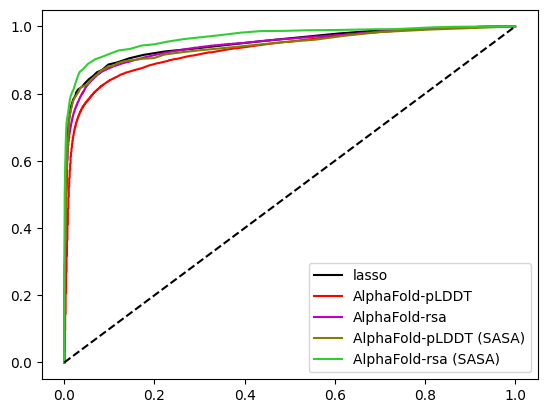
\includegraphics[scale = 0.8]{res/ML/roc-disorderpdb.png}
    \caption{ROC curves - DisorderPDB ground truth}
\end{figure}

\begin{figure}[h!]
    \centering
    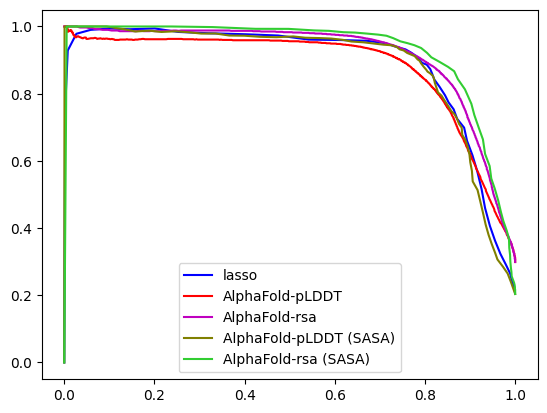
\includegraphics[scale = 0.8]{res/ML/precisionrecall-disorderpdb.png}
    \caption{Precision-Recall curves - DisorderPDB ground truth}
\end{figure}

\pagebreak

\subsection{Disorder NOX}

\begin{figure}[h!]
    \centering
    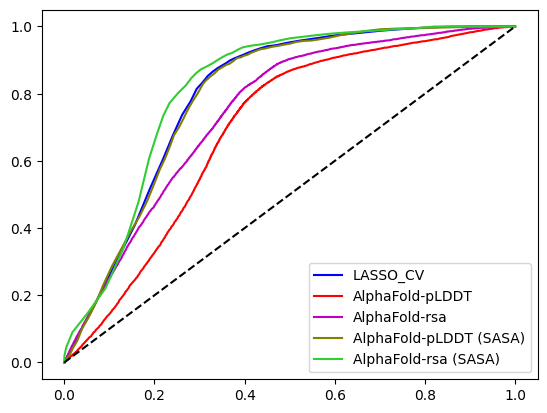
\includegraphics[scale = 0.8]{res/ML/roc-disordernox.png}
    \caption{ROC curves - DisorderNOX ground truth}
\end{figure}



\begin{figure}[h!]
    \centering
    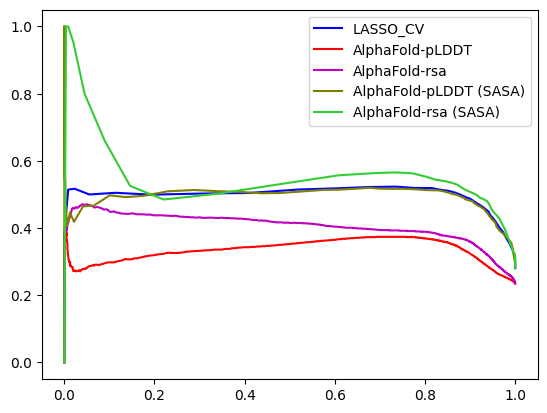
\includegraphics[scale = 0.8]{res/ML/precisionrecall-disordernox.png}
    \caption{Precision-Recall curves - DisorderNOX ground truth}
\end{figure}

\pagebreak

\subsection{Binding}

\begin{figure}[h!]
    \centering
    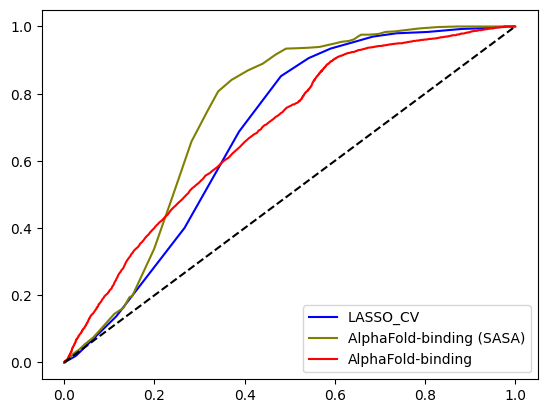
\includegraphics[scale = 0.8]{res/ML/roc-binding.png}
    \caption{ROC curves - Binding ground truth}
\end{figure}

\begin{figure}[h!]
    \centering
    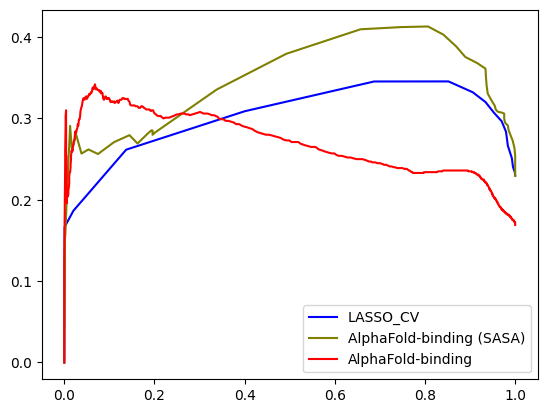
\includegraphics[scale = 0.8]{res/ML/precisionrecall-binding.png}
    \caption{Precision-Recall curves - Binding ground truth}
\end{figure}

\pagebreak

\section{Helper Scripts for Analysis}\label{analysis-procedures}
\subsection{Fetch proteins and functional annotations from DisProt database}
First of all we downloaded the file .json from the DisProt website, in the \href{https://disprot.org/download}{\underline{download page}}. Then we used the library \textbf{json} of Python to extract from the json file, inside the json file we find all the information we want about DisProt proteins. 

Let's quickly analyse the structure of this json: from the root of the json we have two keys, \textbf{data} and \textbf{size}. Size contains just the number of proteins in this json, and data contains an array of DisProt IDs. Each DisProt IDs have several key-value pairs, we are interested in \textbf{acc}, \textbf{disprot\_id} and \textbf{regions}.

We are interested in the key \textbf{'acc'} of every DisProt protein because it is the UniProt ID: with these UniProt IDs we can fetch very quickly all the proteins structure of proteins in DisProt with the AlphaFold database API.
\begin{lstlisting}[language=Python, caption=Script to use AlphaFold database API]
import requests
[...]
list_absent = []
for i in uniprot_ids :
    url = 'https://alphafold.ebi.ac.uk/files/AF-'+i+'-F1-model_v4.pdb'
    r = requests.get(url, allow_redirects=True)
    if r.reason == 'OK' :
        filename = '' + i + '.pdb'
        open(filename,'wb').write(r.content)
    else :
        list_absent.append(i)
        print("Error "+str(r.status_code)+", "+r.reason+": "+i)
\end{lstlisting}

Then we are interested in the functional annotations of every DisProt protein, contained inside the key \textbf{'regions'}:  an array of annotations for that protein.

\pagebreak

\subsection{Fetch ground truths arrays from CAID}
We downloaded the ground truths data from the CAID web site, in the \href{https://caid.idpcentral.org/challenge#Data}{\underline{Data page}}. These ground truth files are in .FASTA, a file format for bioinformatic sequences. 

In these files we have the ground truth for several DisProt ID, and for each of them to each residue is assigned a value between 0, 1 and '-'. '-' means no information, 1 is presence of disorder/binding and 0 is absence.

Finally we parsed these .FASTA files in pandas DataFrames and used them in our analysis. Down below an example of the first rows of the DataFrame for disorder-PDB ground truth.

\begin{table}[h!]
    \centering
    \begin{tabular}{c|c|c|c|c|c}
         & uniprot & disprot & \small amino\_id & amino\_name & disorder-pdb\_GT \normalsize \\
         \hline
        0 & P06837 & DP02342 & 1 & M & 1 \\
        1 & P06837 & DP02342 & 2 & L & 1 \\
        2 & P06837 & DP02342 & 3 & C & 1 \\
        3 & P06837 & DP02342 & 4 & C & 1 \\
        4 & P06837 & DP02342 & 5 & M & 1 \\
        5 & P06837 & DP02342 & 6 & R & 1 \\
    \end{tabular}
    \caption{DataFrame for Disorder-PDB ground truth}
\end{table}